\documentclass[a4paper,oneside,12pt]{extreport}

\usepackage{mmap}
\usepackage[T2A]{fontenc}
\usepackage[utf8]{inputenc}
\usepackage[english,russian]{babel}


% Текст отчёта следует печатать, соблюдая следующие размеры полей:
% левое — 30 мм, правое — 15 мм, верхнее и нижнее — 20 мм.
\usepackage[left=20mm, right=15mm, top=15mm, bottom=15mm]{geometry}

% \setlength{\parindent}{1.25cm} % Абзацный отступ

\usepackage{setspace}
%\onehalfspacing % Полуторный интервал

\frenchspacing % Равномерные пробелы
\usepackage{indentfirst} % Красная строка

\usepackage{microtype}
\sloppy

\usepackage{titlesec}
\titlespacing*{\chapter}{0pt}{-30pt}{8pt}
\titlespacing*{\section}{\parindent}{*4}{*4}
\titlespacing*{\subsection}{\parindent}{*4}{*4}
\titleformat{\chapter}{\LARGE\bfseries}{\thechapter}{20pt}{\LARGE\bfseries}
\titleformat{\section}{\Large\bfseries}{\thesection}{40pt}{\Large\bfseries}

\usepackage{graphicx}
\usepackage{caption}

\usepackage[unicode,pdftex]{hyperref}
\hypersetup{hidelinks}

%% title begin
\usepackage{wrapfig}

\makeatletter
	\def\vhrulefill#1{\leavevmode\leaders\hrule\@height#1\hfill \kern\z@}
\makeatother
%% title end

%% begin code
\usepackage{listings}
\usepackage{xcolor}

\lstset{
	basicstyle=\footnotesize\ttfamily,
	breakatwhitespace=true,
	breaklines=true,
	commentstyle=\color{gray},
	frame=single,
	keywordstyle=\color{blue},
	stringstyle=\color{red},
	tabsize=8
}

\lstdefinestyle{lispinline}{
	frame=none,
	language=Lisp
}

\newcommand{\code}[1]{\texttt{#1}}
%% end code

%% begin theorem
\usepackage{amsthm}

\makeatletter
\newtheoremstyle{indented}
	{}% measure of space to leave above the theorem
	{}% measure of space to leave below the theorem
	{}% name of font to use in the body of the theorem
	{\parindent}% measure of space to indent
	{\bfseries}% name of head font
	{.}% punctuation between head and body
	{ }% space after theorem head; " " = normal interword space
	{}% header specification (empty for default)
\makeatother

\theoremstyle{indented}

\newtheorem{definition}{Определение}[section]
\newtheorem{example}{Пример}[section]
\newtheorem{theorem}{Теорема}[section]
\newtheorem{task}{Задание}

\makeatletter
\DeclareRobustCommand\bfseriesitshape{%
	\not@math@alphabet\itshapebfseries\relax
	\fontseries\bfdefault
	\fontshape\itdefault
	\selectfont
}
\makeatother

\DeclareTextFontCommand{\textbfit}{\bfseriesitshape}
\DeclareTextFontCommand{\define}{\bfseriesitshape}
%% end theorem

%% begin columns
\usepackage{etoolbox,refcount}
\usepackage{multicol}

\newcounter{countitems}
\newcounter{nextitemizecount}
\newcommand{\setupcountitems}{%
	\stepcounter{nextitemizecount}%
	\setcounter{countitems}{0}%
	\preto\item{\stepcounter{countitems}}%
}
\makeatletter
\newcommand{\computecountitems}{%
	\edef\@currentlabel{\number\c@countitems}%
	\label{countitems@\number\numexpr\value{nextitemizecount}-1\relax}%
}
\newcommand{\nextitemizecount}{%
	\getrefnumber{countitems@\number\c@nextitemizecount}%
}
\newcommand{\previtemizecount}{%
	\getrefnumber{countitems@\number\numexpr\value{nextitemizecount}-1\relax}%
}
\makeatother
\newenvironment{AutoMultiColItemize}{%
	\ifnumcomp{\nextitemizecount}{>}{3}{\begin{multicols}{2}}{}%
		\setupcountitems\begin{itemize}}%
		{\end{itemize}%
		\unskip\computecountitems\ifnumcomp{\previtemizecount}{>}{3}{\end{multicols}}{}}
\makeatother
\newenvironment{AutoMultiColEnumerate}{%
	\ifnumcomp{\nextitemizecount}{>}{3}{\begin{multicols}{2}}{}%
		\setupcountitems\begin{enumerate}}%
		{\end{enumerate}%
		\unskip\computecountitems\ifnumcomp{\previtemizecount}{>}{3}{\end{multicols}}{}}
%% end columns

	
\usepackage{amsmath}

\begin{document}

\begin{titlepage}
	{\large % 14pt instead of 12pt
	\onehalfspacing
	\centering

	\begin{wrapfigure}[7]{l}{0.14\linewidth}
		\vspace{3mm}
		\hspace{-10mm}
		
\includegraphics[width=\linewidth]{img/b_logo}
		% \includegraphics[width=0.93\linewidth]{inc/img/bmstu-logo}
	\end{wrapfigure}
	{\singlespacing \footnotesize \bfseries Министерство науки и высшего образования Российской Федерации\\Федеральное государственное бюджетное образовательное учреждение\\высшего образования\\<<Московский государственный технический университет\\имени Н.~Э.~Баумана\\ (национальный исследовательский университет)>>\\(МГТУ им. Н.~Э.~Баумана)\\}

	\vspace{-2.2mm}
	\vhrulefill{0.9mm}\\
	\vspace{-7.5mm}
	\vhrulefill{0.2mm}\\
	\vspace{2mm}

	{\doublespacing \small \raggedright ФАКУЛЬТЕТ \hspace{5mm} \underline{«Информатика и системы управления»}\\
	КАФЕДРА \hspace{10mm} \underline{«Программное обеспечение ЭВМ и информационные технологии»}\\}

	\vspace{20mm}

	\begin{center}
		\noindent\begin{minipage}{1.2\textwidth}\centering
			\textbf{ОТЧЕТ ПО ЛАБОРАТОРНОЙ РАБОТЕ №4}\newline
			\textbf{По курсу: "Моделирование"}\newline\newline\newline
		\end{minipage}
	\end{center}

	\vspace{20mm}

	\noindent ~~Тема \underline{~~~~~Программно-алгоритмическая реализация моделей~~~~~~~~~~~~~~~~~~~~~}\newline
	\underline{~~~~~~~~~~~~~~на основе дифференциальных уравнений в~~~~~~~~~~~~~~~~~~~~~~~~~~~~~~~~~}\newline
	\underline{~~~~~~~частных производных с краевыми условиями II и III рода.~~~~~~~~~~~~~~~~~~}\newline
	\noindent ~~Группа \underline{~~~~~~~~~~~~~~~~~~~~~~~~~~~~~~~~~~~ИУ7-63Б~~~~~~~~~~~~~~~~~~~~~~~~~~~~~~~~~~~~~~~~~~~~~~~~~}\newline
	\noindent ~~Студент \underline{~~~~~~~~~~~~~~~~~~~~~~~~~~~~Сукочева А.~~~~~~~~~~~~~~~~~~~~~~~~~~~~~~~~~~~~~~~~~~~~~~~~~~}\newline
	\noindent ~~Преподаватель \underline{~~~~~~~~~~~~~~~~~Градов В.М.~~~~~~~~~~~~~~~~~~~~~~~~~~~~~~~~~~~~~~~~~~~~~~~~~~~}\newline


	\begin{center}
		\vfill
		Москва~---~\the\year
		~г.
	\end{center}
	}



\end{titlepage}

\setcounter{page}{2}

\section{Постановка задачи}
\textbf{Цель работы}. 
Получение навыков разработки алгоритмов решения задачи Коши при реализации моделей, построенных на системе ОДУ, 
с использованием метода Рунге-Кутта 4-го порядка точности.

\subsection{Исходные данные}

Задана система электротехнических уравнений, описывающих разрядный контур,
включающий постоянное активное сопротивление $R_k$, нелинейное сопротивление $R_p(I)$,
зависящее от тока $I$, индуктивность $L_k$ и емкость $C_k$

\begin{figure}[ht!]
	\centering{
		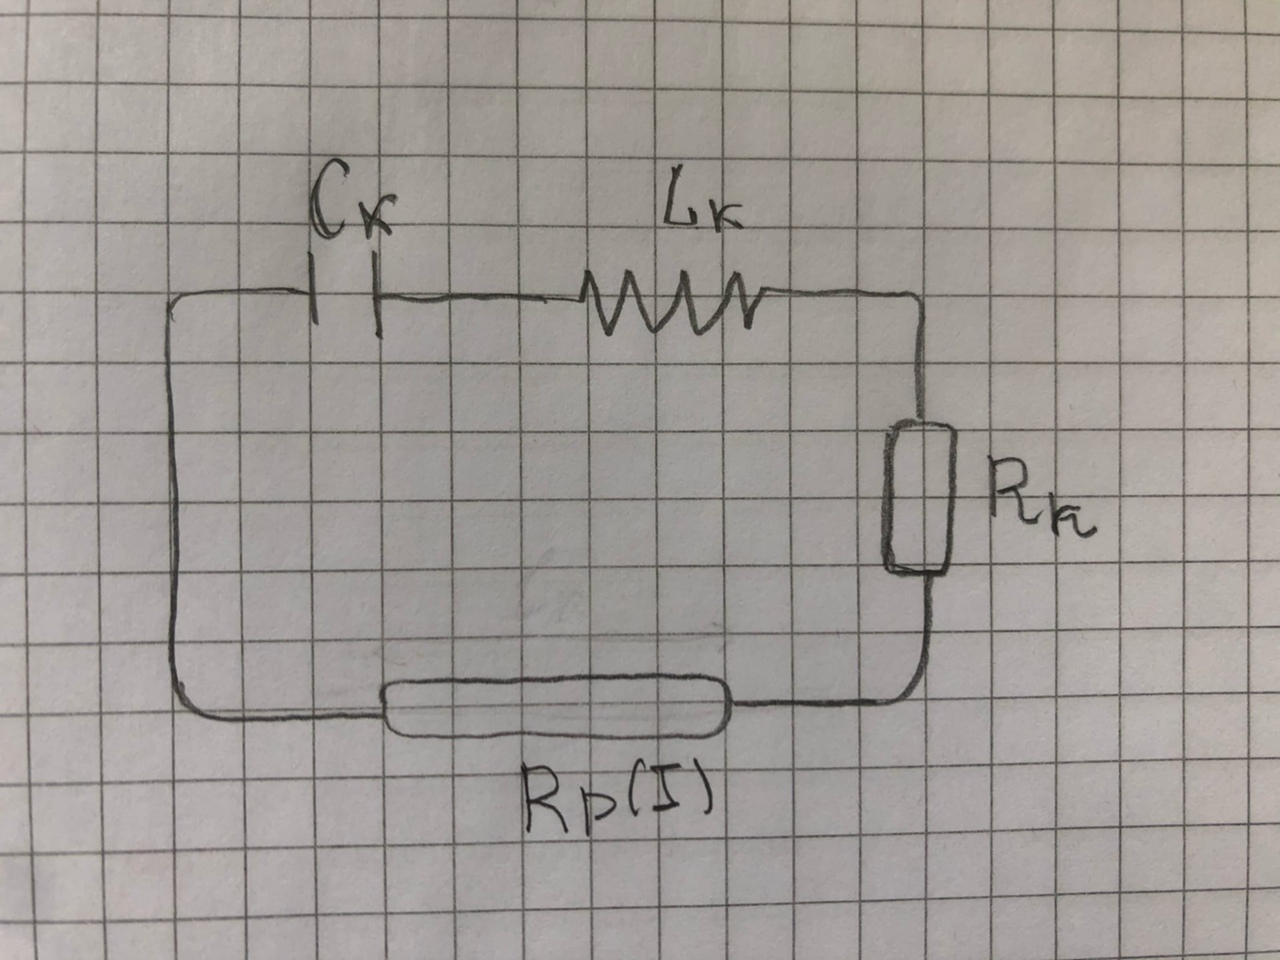
\includegraphics[width=0.6\textwidth]{img/1.jpg}
		\caption{Разрядный контур} }
\end{figure}

\begin{equation*}
     \begin{cases}
        \frac{dI}{dT} = \frac{U - (R_k + R_p(I))I}{L_k} \\ 
        \frac{dU}{dt} = -\frac{I}{C_k} \\ 
     \end{cases}
\end{equation*}

Начальные условия:
\begin{equation*}
t=0, I=I_0, U=U_0
\end{equation*}

Здесь $I$, $U$ - ток и напряжение на конденсаторе.

Сопротивление $R_p$ рассчитать по формуле:

\begin{equation*}
R_p = \frac{l_p}{2 \pi R^2 \int_0^1{\sigma(T(z))zdz}}
\end{equation*}


Для функции $T(z)$ применить выражение
$T(z) = T_0 + (T_w - T_0)z^m$

Параметры $T_0$, $m$ находятся интерполяцией из табл.1 
при известном токе $I$.

Коэффициент электропроводности
$\sigma(T)$ зависит от $T$
и рассчитывается интерполяцией из табл.2.
\begin{center}
Таблица 1
\end{center}
\begin{center}
    \begin{tabular}{ |c||c|c| }
        \hline
     $I$, A & $T_0$, К & $m$ \\ 
     \hline
     \hline
     0.5 & 6730 & 0.50 \\  
     \hline
     1 & 6790 & 0.55 \\  
     \hline
     5 & 7150 & 1.7 \\  
     \hline
     10 & 7270 & 3 \\  
     \hline
     50 & 8010 & 11 \\  
     \hline
     200 & 9185 & 32 \\  
     \hline
     400 & 10010 & 40 \\  
     \hline
     800 & 11140 & 41 \\  
     \hline
     1200 & 12010 & 39 \\  
     \hline
     \hline
    \end{tabular}
\end{center}

\begin{center}
    Таблица 2
\end{center}
\begin{center}
    \begin{tabular}{ |c||c| }
        \hline
        $T$, К & $\sigma$, 1/Ом см\\ 
        \hline
        \hline
        4000 & 0.031\\  
        \hline
        5000 & 0.27 \\  
        \hline
        6000 & 2.05 \\  
        \hline
        7000 & 6.06 \\  
        \hline
        8000 & 12.0 \\  
        \hline
        9000 & 19.9 \\  
        \hline
        10000 & 29.6 \\  
        \hline
        11000 & 41.1 \\  
        \hline
        12000 & 54.1 \\  
        \hline
        13000 & 67.7 \\  
        \hline
        14000 & 81.5 \\  
        \hline
        \hline
    \end{tabular}
\end{center}

Параметры разрядного контура:

$R = 0.35$ см

$l_p = 12$ см

$L_k = 187$ $10^{-6}$ Гн

$C_k = 268$ $10^{-6}$ Ф

$R_k = 0.25$ Ом

$U_{co} = 1400$ В

$I_0 = 0...3$ А

$T_w = 2000$ К


\newpage

\section{Теоретическая часть}

\subsection{ОДУ}

Дано ОДУ (Обыкновенное Дифференциальное уравнение) n-ого порядка (\ref{eq:ody}).

\begin{equation}
	F(x, u', u'', ... , u^{(n)} = 0)
	\label{eq:ody}
\end{equation}

ОДУ любого порядка может быть сведено к системе ОДУ 1-ого порядка.

\subsection{Задача Коши}

\textit{Задача Коши} состоит в нахождении решения дифференциального уравнения, удовлетворяющего начальным условиям. 
Это одна из основных задач теории дифференциальных уравнений.

Имеется задача Коши (\ref{eq:ref1}).

\begin{equation}
	{\begin{cases}
			u'(x) = f(x,u) \\
			u(\xi) = \eta
		\end{cases}}
		\label{eq:ref1}
\end{equation}

Методы решения ОДУ в задачи Коши:

\begin{enumerate}
	\item аналитические;
	\item приближенно аналитические;
	\item численные.
\end{enumerate}

\subsection{Метод Рунге-Кутта четвертого порядка точности}

Преимущества схем Р-К.
\begin{enumerate}
    \item Достаточно точные.
    \item Легко изменить шаг.
    \item Методы не требуют перехода к другим методам.
    \item Явные.
\end{enumerate}

Дана система уравнений вида:

\begin{equation}
	{\begin{cases}
			u'(x) = f(x,u,v) \\
			v'(x) = \phi(x,u,v) \\
			u(\xi) = \eta_1 \\
			v(\xi) = \eta_2
		\end{cases}}
		\label{eq:ref1}
\end{equation}

Тогда 

\begin{equation*}
    y_{n+1} = y_n + \frac{k_1+2k_2+2k_3+k_4}{6}
\end{equation*}
    
\begin{equation*}
    z_{n+1} = z_n + \frac{p_1+2p_2+2p_3+p_4}{6}
\end{equation*}

, где

\begin{equation*}
    k_1 = hf(x_n,y_n,z_n)
\end{equation*}

\begin{equation*}
    k_2 = hf(x_n + \frac{h}{2},y_n+\frac{k_1}{2},z_n+\frac{p_1}{2})
\end{equation*}

\begin{equation*}
    k_3 = hf(x_n + \frac{h}{2},y_n+\frac{k_2}{2},z_n+\frac{p_2}{2})
\end{equation*}

\begin{equation*}
    k_4 = hf(x_n + h,y_n+k_3,z_n+p_3)
\end{equation*}


\begin{equation*}
    p_1 = h\phi(x_n,y_n,z_n)
\end{equation*}

\begin{equation*}
    p_2 = h\phi(x_n + \frac{h}{2},y_n+\frac{k_1}{2},z_n+\frac{p_1}{2})
\end{equation*}

\begin{equation*}
    p_3 = h\phi(x_n + \frac{h}{2},y_n+\frac{k_2}{2},z_n+\frac{p_2}{2})
\end{equation*}

\begin{equation*}
    p_4 = h\phi(x_n + h,y_n+k_3,z_n+p_3)
\end{equation*}

\section{Экспериментальная часть}


\subsection{Номер 1}
\subsection{Номер 2}
\subsection{Номер 3}

\subsection{Номер 4}

Результаты исследования влияния параметров контура
$C_k$, $L_k$, $R_k$ на длительность импульса tимп. апериодической формы.
Длительность импульса определяется по кривой зависимости тока 
от времени на высоте 0.35 *  $I_{max}$  , $I_{max}$ - значение тока в максимуме.

Для исследования влияния параметров контура на длительность импульса tимп
будем использовать приведенный ниже код.

\begin{lstlisting}
    double Imax = arr_I.Max();
    double pulseDuration = arr_I.Count(I => I > Imax * 0.35);
\end{lstlisting}

\subsection{Исследование влияния $C_k$ на длительность импульса.}

Из приведенного исследования видно, что при увеличении $C_k$
длительность импульса увеличивается, а при уменьшении $C_k$
длительность импульса уменьшается.


\begin{figure}[ht!]
	\centering{
		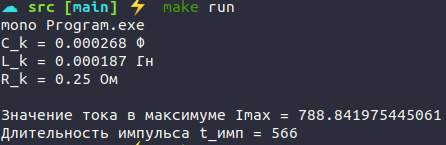
\includegraphics[width=0.6\textwidth]{img/task4/ck_1.png}
		\caption{Исследование влияния $C_k$ на длительность импульса tимп.  } }
\end{figure}

\begin{figure}[ht!]
	\centering{
		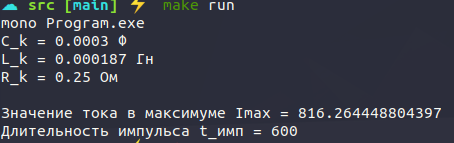
\includegraphics[width=0.6\textwidth]{img/task4/ck_2.png}
		\caption{Исследование влияния $C_k$ на длительность импульса tимп.  } }
\end{figure}

\begin{figure}[ht!]
	\centering{
		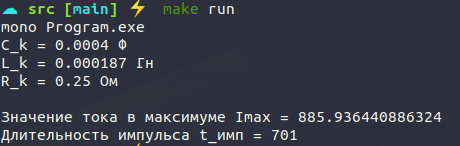
\includegraphics[width=0.6\textwidth]{img/task4/ck_3.png}
		\caption{Исследование влияния $C_k$ на длительность импульса tимп.  } }
\end{figure}

\begin{figure}[ht!]
	\centering{
		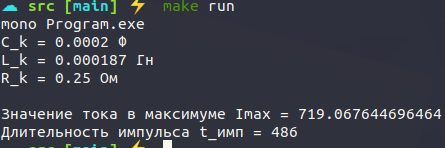
\includegraphics[width=0.6\textwidth]{img/task4/ck_4.png}
		\caption{Исследование влияния $C_k$ на длительность импульса tимп.  } }
\end{figure}


\subsection{Исследование влияния $L_k$ на длительность импульса.}

Из приведенного исследования видно, что при увеличении $L_k$
длительность импульса увеличивается, а при уменьшении $L_k$
длительность импульса уменьшается.

\begin{figure}[ht!]
	\centering{
		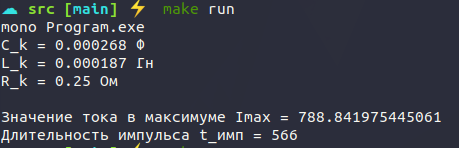
\includegraphics[width=0.6\textwidth]{img/task4/lk_1.png}
		\caption{Исследование влияния $L_k$ на длительность импульса tимп.  } }
\end{figure}

\begin{figure}[ht!]
	\centering{
		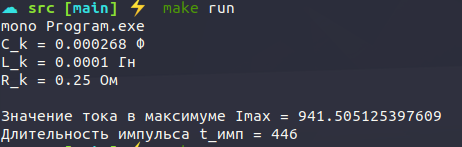
\includegraphics[width=0.6\textwidth]{img/task4/lk_2.png}
		\caption{Исследование влияния $L_k$ на длительность импульса tимп.  } }
\end{figure}

\begin{figure}[ht!]
	\centering{
		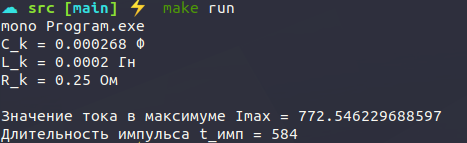
\includegraphics[width=0.6\textwidth]{img/task4/lk_3.png}
		\caption{Исследование влияния $L_k$ на длительность импульса tимп.  } }
\end{figure}

\begin{figure}[ht!]
	\centering{
		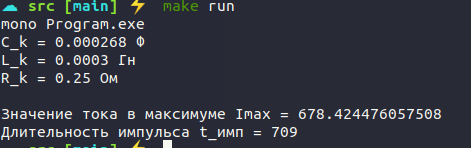
\includegraphics[width=0.6\textwidth]{img/task4/lk_4.png}
		\caption{Исследование влияния $L_k$ на длительность импульса tимп.  } }
\end{figure}

\subsection{Исследование влияния $R_k$ на длительность импульса.}

Из приведенного исследования видно, что при увеличении $R_k$
длительность импульса увеличивается, а при уменьшении $R_k$
длительность импульса уменьшается.

\begin{figure}[ht!]
	\centering{
		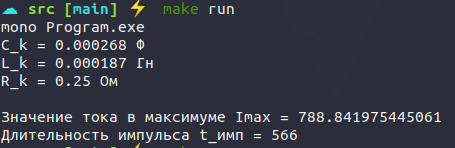
\includegraphics[width=0.6\textwidth]{img/task4/rk_1.png}
		\caption{Исследование влияния $R_k$ на длительность импульса tимп.  } }
\end{figure}

\begin{figure}[ht!]
	\centering{
		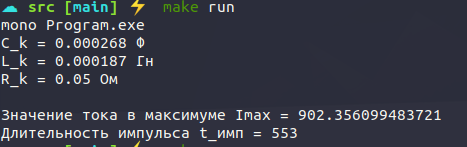
\includegraphics[width=0.6\textwidth]{img/task4/rk_2.png}
		\caption{Исследование влияния $R_k$ на длительность импульса tимп.  } }
\end{figure}

\begin{figure}[ht!]
	\centering{
		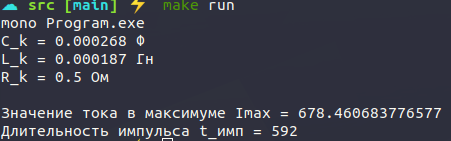
\includegraphics[width=0.6\textwidth]{img/task4/rk_3.png}
		\caption{Исследование влияния $R_k$ на длительность импульса tимп.  } }
\end{figure}

\end{document}